% Chapter Template

\chapter{Extending the Test Framework} % Main chapter title
\label{Chapter4}

Talk about why we changed the WiFi definition 
Strength and weaknesses
Realised there were difficulties with that
Present the first approach
List the weaknesses, 


\section{Joint WiFi \& Radio Tests}
A key part of the test framework that was missing was support for networks with both WiFi and radio link types. 
This presents a major limitation  to the test framework as the vast majority of real Serval networks would feature both of these network links.
To implement this feature, several additions need to be made to the test framework.

First, the ability to define which link will be used for each node needs to be defined.
This will allow test definition writers to define the connectivity of each of the nodes. 
For instance, this allows testers to define a WiFi connection between two nodes or a radio connection using the RFD900.

Next, the ability to define specific network topologies will need to be added.
This already exists in the case of the Fakeradio networks as discussed in the previous chapters, however this is not as easily done with simulated WiFi connections.

Once these two pieces of functionality have been added to the test framework, developers will be able to test considerably larger and more complicated network topologies with ease.
With this expanded test framework the Serval team will be able to significantly increase their test coverage for the Serval network.


To achieve this, several features need to be implemented. 
The first feature is defining the interfaces to be used on a per-node basis.
With this, nodes can each have their own configuration, allowing for some nodes to have WiFi enabled while others only have Fakeradio interfaces.
Next, the ability to define WiFi topologies will need to be added, as currently it appears to only be possible to have nodes communicating with every other node without any defined topology.

To ensure that this does not affect pre-existing LBARD tests, two new files will be created.
The first is the \verb|topologies| test file.
This file is just a new test file written in bash that outlines the new tests to be implemented.
Next, as these topology tests will need to use some overwritten test definitions from the original \texttt{testdefs.sh} file, a new test definition file (\texttt{topology\_testdefs.sh}) will be created that extends these functions.



\subsection{Defining interfaces per node}
To allow for some nodes to support WiFi only, while others communicate over just radio, and others again use both, specific network interfaces will need to be enabled on a per-node basis.
Before this is added, all Serval nodes in a test use the exact same configuration as defined in the test definition.
By implementing per-node configuration, the test framework will be able to enable WiFi and radio interfaces on some nodes while disabling them on others, allowing for complicated mixed-link network topologies to be run and tested.

The first step to completing this is to determine what nodes need which configuration applied.
Two possibilities exist for this; manually define the configurations for each node in the test definition or automatically determine which configuration is required for each node.
Since each node that will be connected by Fakeradio needs to be defined already, it was decided to use this information to determine what configuration the node needed.

Each test that uses Fakeradio contains a string in the setup function defining the links between nodes.
An example of this is shown in \todo{add figure}. 
The string defines the links in the format "allow between [n],[m];" where n and m are the 0-indexed serval-dna instance number.
This is suitable to use since every node in a topology using Fakeradio must be specified in this string, meaning that every node that requires LBARD interfaces defined will be listed here.
As the WiFi functionality does not need to have the topology defined in such a way it is necessary to define a new string, simply listing the nodes that require WiFi to be enabled. 

These strings are passed to the \verb|start\_instances| function. 
To determine what nodes to enable the configurations on, the node information needs to be stripped from the string.


To achieve this, both of these strings are altered to extract just the 0-indexed instance numbers which are then assigned to an array of integers.
This results in two arrays (WiFi and Fakeradio) of the instance numbers.
With this information, we can now programmatically determine which configurations need to be enabled on each node.

To do this, the program simply creates a new array of the instances required for each node.
It does this by iterating through both the WiFi and Fakeradio arrays and appends either "wifi" or "fakeradio" to the array at the position of the instance number.
The end result is that at the index of the instance number a string lists what interfaces are required for this node: "wifi", "fakeradio" or "wifi fakeradio".

The framework then iterates through every node and sends the string containing the needed interfaces to the \verb|configure\_servald\_server| function.


The \verb|configure\_servald\_server| function is called for each node before the instance is started, and as such each configuration is unique to each instance of Servald.
This means that we can now add the required configuration for a node without affecting other nodes.
When the configure\_servald\_server function is called, the program simply calls the \verb|add\_servald\_interface| function with the interfaces needed for that given node.
When this is called the program iterates through the supplied interfaces (i.e. 'wifi', 'fakeradio', or 'fakeradio wifi') and for each interface configures the Servald instance appropriately.
For Fakeradio instances, the only configuration that needs to be set is enabling HTTP (to connect to LBARD) and setting the username and password for LBARD.

With this completed, it is now possible to run WiFi and Fakeradio nodes side-by-side, with the appropriate interfaces enabled based on the test definition.
However, this method has a major limitation; it is not possible to have complicated WiFi topologies with this method since WiFi nodes have zero restriction around what other WiFi nodes they can communicate with.
This means that while networks such as \todo{figure a; A-r-B-w-C-r-D} work, any network such as \todo{figure b} will not work as there is no way to restrict node E from connecting to node C.



\subsection{Defining WiFi topologies}
When expanding the test framework to handle the mixed topologies, it was planned to implement functionality to define WiFi network layouts in the same format as defining Fakeradio networks, however it was suggested to instead define WiFi interfaces using the existing tools found in the Serval-DNA framework.
While this meant that topology tests would not have a consistent method of defining network layouts between radio and WiFi nodes, it would however be consistent with Serval-DNA tests.

Using the method previously outlined in the previous section, WiFi nodes all default to using the same WiFi interface — thus creating a fully-connected WiFi mesh sub-network, leading to every WiFi node being connected with every other WiFi node.
This can be seen in \figurename{ \ref{fig:networkWifi1}}.
Each WiFi interface is essentially a sub-network, with nodes within a specified interface only able to communicate with nodes within the same interface as themselves.
Thus, to define a complicated network topology it is necessary to restrict which interfaces WiFi nodes can communicate on.

\begin{figure}
    \begin{centering}
        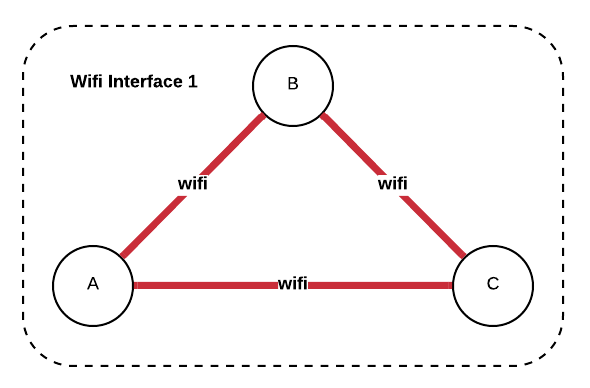
\includegraphics[width=14cm,height=20cm,keepaspectratio]{Figures/networkWifiInterface1.png}
        \caption{Network topology without defining interfaces}
        \label{fig:networkWifi1}
    \end{centering}
\end{figure}

In the Serval-DNA test framework, non- fully-connected WiFi networks are created by manually defining the WiFi interfaces that a specified Servald interface is connected to.
To implement this, several changes need to be made.
The first is removing the functions added in the previous section that relate to WiFi.
This is because we'll no longer be defining WiFi nodes with a string passed to the setup functions.
Next, it was decided for every node to automatically have WiFi functionality enabled by default, but only connected to its own private interface as this more accurately represents how real Serval nodes act in real usage \todo{ref}.
This is done by changing the configuration parsing added in the previous section to enable WiFi by default, but still only enabling LBARD as specified.

To connect nodes via WiFi they must now be connected to a specific WiFi interface as shown in the example test definition \figurename{ \ref{fig:definingInterfaces}}.


\lstset{language=bash,
showstringspaces=false,
numbers=left,
}

\begin{figure}
    \begin{centering}
        \begin{lstlisting}[breaklines, frame=single]
doc_DualType="A 4 node wifi/rfd900 chain. One wifi, two radio links"
setup_DualType(){
    # A -r-> B -w-> C -r-> D
    # No radio connection between 1(B) and 2(C)
    lbardparams="allow between 0,1; allow between 2,3; deny all;"

    setup 0 0 0 "\${lbardparams}"
    # Connect 1(B) and 2(C) via a wifi/rhizome interface of number 1
    foreach_instance +B +C add_servald_interface 1

    # Insert a file to server A
    set_instance +A
    rhizome_add_file file1 50
}
test_DualType(){
    dReceivedBundles() {
        bundle_received_by $BID:$VERSION +D
    }
    wait_until --timeout=60 dReceivedBundles
}
        \end{lstlisting}
        \caption{Example of test definition}
        \label{fig:definingInterfaces}
    \end{centering}
\end{figure}

Using this method, a node is able to communicate with every other node that uses the same WiFi interfaces as it.
As a node can be assigned multiple WiFi interfaces, this allows for network topologies that are more complicated than simple fully-connected mesh networks, such as chains of WiFi nodes as shown in \figurename{ \ref{fig:networkWifi2}}.

\begin{figure}
    \begin{centering}
        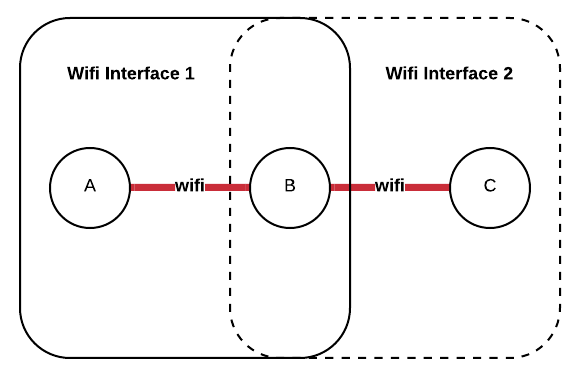
\includegraphics[width=14cm,height=20cm,keepaspectratio]{Figures/networkWifiInterface2.png}
        \caption{Network topology with two WiFi interfaces defined}
        \label{fig:networkWifi2}
    \end{centering}
\end{figure}


\section{Implementing easier network definition}
To assist with creating complex network topologies, a function \verb|setupN| was implemented that allowed for an arbitrary number of Servald and LBARD instances to be created and networked together.
This function is needed as the LBARD test framework lacked any way of defining an arbitrary number of nodes and instead only provides function to start 4 or 10 Servald devices.
As such, a function that can create and start an arbitrary number of nodes is crucial for the expansion of the LBARD test framework.

This \verb|setupN| function accepts four parameters; a string of node characters, a string of radio types ('none' if LBARD is not to be started on the relevant node), the Fakeradio parameters (i.e. packet loss), and finally the parameters for each LBARD instance.
This function then starts a Servald process on each of these nodes, and if defined in the string of radio types, starts LBARD with the specified radio interface on the same node.
Once Servald and LBARD is running on every relevant node with the appropriate configurations as outlined in the previous sections, the function then starts \verb|fakeradio| as necessary.

With this function implemented, the testing capabilities of the LBARD test framework have dramatically increased.
By using this function, testers are able to easily define and test the exact number of Serval nodes that they require in their test, and with the capability to define exact parameters of the test — such as defining which radio to use on a per-node basis and packet loss — this relatively simply function presents a huge increase in testability.
Furthermore, this function when combined with the implementation of mixing WiFi and Fakeradio interfaces allows for Serval testers to test a far greater number of Serval networks with ease.


\section{Adding more topologies tests}
With the improvements made to the LBARD test framework, several new topology tests can be implemented to test the functionality of LBARD in various different network topologies.
The implemented topology tests do not all strictly need to feature WiFi alongside radio, as any test which focuses on a specific network topology that did not exist previously represents an expansion of the test framework.
All of these tests were implemented using the functionality developed throughout this chapter, and followed the same process of adding tests as outlined in section \todo{Link to chapter 3}.
The tests that have been implemented are found in the following table.
\begin{table}[h!]
    \centering
    \begin{tabularx}{\textwidth}{l|X}
        \textbf{Name:}  &  \textbf{Description} \\ \hline
        DualType            &   A chain of 4 nodes, with A and B, and C and D connected with a RFD900 interface, and B and C connected over WiFi. A has a bundle. Finishes when D receives bundle \\ \hline
        RFD900 Chain    &   A chain of 10 RFD900 connected nodes. A has a 100 byte bundle. Finishes when J receives the bundle   \\ \hline
        WiFi\_RFD900\_Chain\_Short & A chain of 5 nodes with alternating UHF/WiFi links. A has a 100 byte bundle. Finishes when F receives the bundle. \\ \hline
        Wifi\_RFD900\_Chain & A chain of 5 nodes with alternating UHF/WiFi links. A has a 100 byte bundle. Finishes when J receives the bundle.     \\ \hline
        LBARD\_Big\_File\_Chain & 4 RFD900 nodes in a chain. A has a 5kb file. Ends when D receives the file.  \\ \hline
        Lab\_File   & Emulated Tonsley lab network. Node A (Lab node) has a file. Ends when H (node A3) receives the file.  \\ \hline
        Lab\_Message& Tonsley lab network topology. Simulates a MeshMS conversation between C (Tonsley node 9) and H (Tonsley node A3). Ends when C receives the final message from H.   \\ \hline
        SplitRFD900 & 5 RFD900 nodes. A can communicate with B, C, and D. E communicate with B, C, D only. A has a 50 byte file. Ends when E receives the whole file. \\ \hline        
    \end{tabularx}
\end{table}
The test that have been implemented represent a significant addition to the testing coverage of the test framework.
While the developed tests are not exhaustive, they provide a valuable groundwork for the further expansion of the test coverage.
The tests cover a wide range of test cases, with the developed tests focusing on how Serval networks handle communication through complicated network topologies.
This is most obvious in both of the Lab tests. These tests model the real-world lab network that the Serval team have set up at the Flinders University Tonsley campus.
In these tests, the reliability of LBARD is tested, particularly in the LBARD\_Big\_File\_Chain test, where a large file is sent across several RFD900 hops.
Further, these tests analyse how LBARD handles a single node receiving bundle pieces from several nodes at a time, notably in SplitRFD900 and both of the Tonsley lab tests.


\begin{itemize}
    \item Complicated topologies (find some that represent real models and reference) \todo{add}
    \item ‘Island’ networks where clusters of nodes communicated over a short-range link such as WiFi or UHF and then communicated via a long-range link such as HF or satellite radio to another cluster. \todo{add this test}
\end{itemize}




\pagebreak
\section{Summary}
In this chapter the testing capability of the Serval network has been significantly increased.
This was done by three different methods.
The first was the implementation of allowing the test framework to handle multiple different interfaces.
With the implementation of this, future tests are able to support a mixed network topology, with the ability now present to have tests where nodes can communicate over both WiFi and radio. 

In this chapter, the test framework was further improved by increasing the ease of defining networks using the framework.
This was done by providing the ability to easily define the exact number and configuration of nodes for the test.
This allows testers a far greater level of control over the parameters of the test, thus allowing them to test networks more easily and more effectively.

Finally, these improvements to the test framework were utilised to add significantly more topology-focused tests.
Using these improvements to expand the test coverage serves a dual purpose: first, the Serval network is more thoroughly tested, and secondly, the newly created improvements are themselves tested by being used and their usefulness demonstrated.

While these improvements have significantly enhances the Serval test framework, there are still some issues with it.
The foremost issue is the output of the test framework; the format is inconsistent, and due to the nature of how the test framework structures the test output is difficult to analyse how a network performed during a test.
To address this, in the next chapter we will analyse the limitations around the output, and implement several improvements to this output.